\section{Support Vector Machines}
\subsection*{Decision Boundary}
The decision boundary of a SVM can be defined as:\\
$w_1x_1 + w_2x_w + b = 0$\\
General form:\\
$\mathbf{w}\cdot\mathbf{x} + b = 0$\\
\subsection*{Making predictions}
During training, the values of $\mathbf{w}$ and $b$ is learned.\\\\
For any test example $\mathbf{x}^*$\\
\[\begin{cases}
    f(\mathbf{x}^*) = +1, \text{if} \mathbf{w}\cdot\mathbf{x}^*+b\geq0\\
    f(\mathbf{x}^*) = -1, \text{if} \mathbf{w}\cdot\mathbf{x}^*+b<0
\end{cases}\]
\subsection*{Other notes (Linear Algebra):}
\textbf{Inner Product}\\
\[\mathbf{u} \cdot \mathbf{v} = \sum^{d}_{i=1}(u_i\times v_i) \]
\[\mathbf{u} \cdot \mathbf{v} = ||\mathbf{u}||_2\times||\mathbf{v}||_2\times cos(\theta) \]

\textbf{L2 Norm (Length of vector)}
\[||\mathbf{u}||_2 = \sqrt{\mathbf{u}\cdot\mathbf{u}} = \sqrt{\sum^{d}_{i=1}(u_i\times u_i)} \]
\subsection*{Induction}
- Direction of $\mathbf{w}$ is orthogonal (perpendicular) to the decision boundary.\\\\
Parallel hyperplanes:\\
$\mathbf{w}\cdot\mathbf{x} + b = k$\\
$\mathbf{w}\cdot\mathbf{x} + b = -k$\\
(After rescaling $\mathbf{w} = \mathbf{w}/k$, $b = b/k$)\\
$\mathbf{w}\cdot\mathbf{x} + b = 1$\\
$\mathbf{w}\cdot\mathbf{x} + b = -1$\\\\
\[||\mathbf{w}||_2 \times d = 2\]
\[d=\frac{2}{||\mathbf{w}||_2}\]
\subsection*{Margin Maximisation}
Therefore, decision boundary can be learnt by maximising the margin, $d=\frac{2}{||\mathbf{w}||_2}$. However, this is not easy.
Change this into a minimisation problem.\\
Minimise: $\frac{||\mathbf{w}||_2^2}{2}$\\
Constraints:\\
$\mathbf{w}\cdot\mathbf{x}_i + b \geq 1, \text{if} y_i = 1$\\
$\mathbf{w}\cdot\mathbf{x}_i + b \leq -1, \text{if} y_i = -1$\\
OR, $y_i \times (\mathbf{w}\cdot\mathbf{x}_i + b) \geq 1$
\subsection*{Optimisation Problem for SVM}
\[min_{w,b} \frac{||\mathbf{w}||_2^2}{2}\]
\[\text{s.t.} y_i \times (\mathbf{w}\cdot\mathbf{x}_i + b) \geq 1\]
\subsection*{Multi-Class SVM}
Given 3-class problem $C_1$, $C_2$ and $C_3$\\
Create 3 SVM binary classifiers:
1. Positive $C_1$, Negative $C_2$ \& $C_3$\\
2. Positive $C_2$, Negative $C_1$ \& $C_3$\\
3. Positive $C_3$, Negative $C_1$ \& $C_2$\\\\
Use majority voting to determine class for test example.
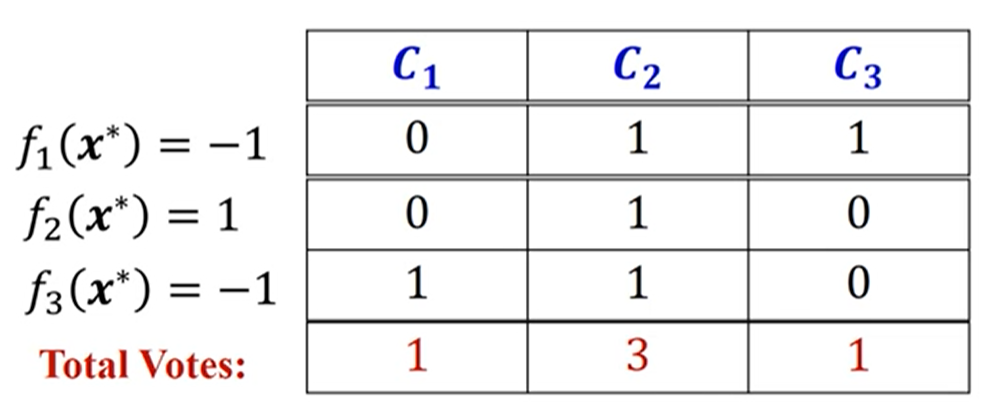
\includegraphics[width=\linewidth]{fig/multiclasssvm.PNG}

